\section{The Degree of a Vertex}
There are many numbers, referred to as \bf{parameters}, associated with a graph $G$. Knowing the values of certain parameters provides us with information about $G$ but rarely tells us the entire structure of $G$. (These comments are tied in with the concept of isomorphic graphs, which will be discussed in Chapter 3.) We've already mentioned the best known parameters: the order and the size. There are also numbers associated with each vertex of a graph. We now consider the best known of these.

The \bf{degree of a vertex} $v$ in a graph $G$ is the number of edges incident with $v$ and is denoted by $\deg{G}{v}$ or by $\deg{}{v}$ if the graph $G$ is clear from the context. Also, $\deg{}{v}$ is the number of vertices adjacent to $v$. Recall that two adjacent vertices are referred to as neighbors of each other. The set $N(v)$ of neighbors of a vertex $v$ is called the \bf{neighborhood} of $v$. Thus $\deg{}{v} = |N(v)|$.

A vertex of degree 0 is referred to as an \bf{isolated vertex} and a vertex of degree 1 is an \bf{end-vertex} (or a \bf{leaf}). The \bf{minimum degree} of $G$ is the minimum degree among the vertices of $G$ and is denoted $\delta(G)$; the \bf{maximum degree} of $G$ is denoted by $\Delta(G)$. So if $G$ is a graph of order $n$ and $v$ is any vertex of $G$, then
\begin{align*}
0 \leq \delta(G) \leq \deg{}{v} \leq \Delta(G) \leq n-1.
\end{align*}
The graph $G$ of Figure 2.1 has order 6 and size 5. Each vertex of $G$ is labeled with its degree. Since $G$ contains an isolated vertex, namely $u$, it follows that $\delta(G) = 0$. Furthermore, $w$ has the largest degree in $G$ and so $\Delta(G) = \deg{}{w} = 4$. Both $v$ and $z$ are end-vertices of $G$ since $\deg{}{v} = \deg{}{z} = 1$. If we add the degrees of the vertices of $G$, we obtain $0+1+1+2+2+4=10$, which happens to be twice the size of $G$. This is not a coincidence as we show in our next theorem, which is often referred to as \bf{The First Theorem of Graph Theory}, so-called because it is likely that anyone studying graph theory for the first time would discover this result as his or her own first theorem on the subject. Although we've already discovered some theorems in Chapter 1, we'll follow the trend and also refer to the following theorem as the First Theorem of Graph Theory.

\begin{figure}[h]
	\caption{A graph $G$ with $\delta(G)=0$ and $\Delta(G)=4$}
\end{figure}

\begin{thm}[The First Theorem of Graph Theory]
If $G$ is a graph of size $m$, then
\begin{align*}
\sum\limits_{v \in V(G)} \deg{}{v} = 2m.
\end{align*}
\end{thm}

\begin{pf}
When summing the degrees of the vertices of $G$, each edge of $G$ is counted twice, once for each of its two incident vertices.
\end{pf}

The First Theorem of Graph Theory is useful in solving problems such as the following.

\begin{exmp}\let\qed\relax
A certain graph $G$ has order 14 and size 27. The degree of each vertex of $G$ is 3, 4 or 5. There are six vertices of degree 4. How many vertices of $G$ have degree 3 and how many have degree 5?
\end{exmp}

\begin{soln}
Let $x$ be the number of vertices of $G$ having degree 3. Since the order of $G$ is 14 and six vertices have degree 4, eight vertices have degree 3 or 5. So there are $8-x$ vertices of degree 5. Summing the degrees of the vertices of $G$ and applying the First Theorem of Graph Theory, we obtain
\begin{align*}
3 \cdot x + 4 \cdot 6 + 5 \cdot (8-x) &= 2 \cdot 27 \\
3x + 24 + 40 - 5x &= 54 \\
-2x &= -10 \\
x &= 5
\end{align*}
and so $8-x = 3$. Thus $G$ has five vertices of degree 3 and three vertices of degree 5.
\end{soln}

The method we used to solve the problem in Example 2.2 tells us that there is a unique solution. Perhaps other methods of solving this problem might have occurred to you, such as trying to draw the graph. Consider the graph of Figure 2.2, each of whose vertices is labeled by its degree. This graph has order 14, size 27 and six vertices of degree 4, which are characteristics of the graph $G$ of Example 2.2. We see that the graph of Figure 2.2 has five vertices of degree 3 and three vertices of degree 5, solving the problem. Even though this provides the correct answers to our question, the explanation is not correct; for how do we know that the graph we have just drawn is \it{the} graph $G$ referred to in the problem and therefore gives us the correct answer?

\begin{figure}[h]
	\centering
	\begin{tikzpicture}
		\vertex (0) at (0,0) [label=210:$5$]{};
		\vertex (1) at (30:1) [label=0:$5$]{};
		\vertex (2) at (90:1) [label=60:$4$]{};
		\vertex (3) at (150:1) [label=180:$5$]{};
		\vertex (4) at (210:1) [label=210:$4$]{};
		\vertex (5) at (270:1) [label=270:$4$]{};
		\vertex (6) at (330:1) [label=330:$4$]{};
		\vertex (7) at (90 - 360 / 7:2) [label=90 - 360 / 7:$3$]{};
		\vertex (8) at (90:2) [label=90:$3$]{};
		\vertex (9) at (90 + 360 / 7:2) [label=90 + 360 / 7:$3$]{};
		\vertex (10) at (90 + 2 * 360 / 7:2) [label=90 + 2 * 360 / 7:$4$]{};
		\vertex (11) at (90 + 3 * 360 / 7:2) [label=90 + 3 * 360 / 7:$4$]{};
		\vertex (12) at (90 + 4 * 360 / 7:2) [label=90 + 4 * 360 / 7:$3$]{};
		\vertex (13) at (90 + 5 * 360 / 7:2) [label=90 + 5 * 360 / 7:$3$]{};
		\path
			(0) edge (1)
			(0) edge (2)
			(0) edge (3)
			(0) edge (5)
			(0) edge (6)
			(1) edge (2)
			(1) edge (6)
			(1) edge (7)
			(1) edge (13)
			(2) edge (3)
			(2) edge (8)
			(3) edge (4)
			(3) edge (9)
			(3) edge (10)
			(4) edge (5)
			(4) edge (10)
			(4) edge (11)
			(5) edge (6)
			(5) edge (11)
			(6) edge (12)
			(7) edge (8)
			(7) edge (13)
			(8) edge (9)
			(9) edge (10)
			(10) edge (11)
			(11) edge (12)
			(12) edge (13)
		;
	\end{tikzpicture}
	\caption{A graph of order 14 and size 27}
\end{figure}

Another possible "solution" might go something like this: We know that we are looking for integers $x$ and $y$ such that $x+y=8$ and
\begin{align*}
3x + 4 \cdot 6 + 5y = 2 \cdot 27 = 54.
\end{align*}
By observation, we see that $x=5$ and $y=3$ satisfy this equation. Thus we have "solved" the problem. But this "solution" also has its drawbacks. How do we know that this is the \it{only} solution? (Of course, we could try all possible values of $x$ and $y$.) The solution that we gave for Example 2.2 shows that there is only one solution for each of $x$ and $y$ and that the solutions do not depend on the graph under consideration (provided it has order 14, size 27 and six vertices of degree 4). Just as when asked to solve $x^{2}-x=3x-4$ for a real number $x$, it is not enough to simply note that $x=2$ is a root. It is required to find \it{all} roots and even if $x=2$ is the \it{only} root, we are obliged to show this is so.

Suppose that $G$ is a bipartite graph of size $m$ with partite sets $U = \{u_{1},u_{2},\ldots,u_{s}\}$ and $W = \{w_{1},w_{2},\ldots,w_{t}\}$. Since every edge of $G$ joins a vertex of $U$ and a vertex of $W$, it follows that adding the degrees of the vertices in $U$ (or in $W$) gives the number of edges in $G$, that is,
\begin{equation}
\sum\limits_{i=1}^{s} \deg{}{u_{i}} = \sum\limits_{j=1}^{t} \deg{}{w_{j}} = m.
\end{equation}

A vertex of even degree is called an \bf{even vertex}, while a vertex of odd degree is an \bf{odd vertex}. Returning to the graph $G$ of Figure 2.2, we see that it has six even vertices and eight odd vertices. In particular, the number of odd vertices of $G$ is even. We show that this is the case for every graph.

\begin{cor}
Every graph has an even number of odd vertices.
\end{cor}

\begin{pf}
Let $G$ be a graph of size $m$. Divide $V(G)$ into two subsets $V_{1}$ and $V_{2}$, where $V_{1}$ consists of the odd vertices of $G$ and $V_{2}$ consists of the even vertices of $G$. By the First Theorem of Graph Theory,
\begin{align*}
\sum\limits_{v \in V(G)} \deg{}{v} = \sum\limits_{v \in V_{1}} \deg{}{v} + \sum\limits_{v \in V_{2}} \deg{}{v} = 2m.
\end{align*}
The number $\sum_{v \in V_{2}} \deg{}{v}$ is even since it is a sum of even integers. Thus
\begin{align*}
\sum\limits_{v \in V_{1}} \deg{}{v} = 2m - \sum\limits_{v \in V_{2}} \deg{}{v},
\end{align*}
which implies that $\sum_{v \in V_{1}} \deg{}{v}$ is even. Since each of the numbers $\deg{}{v}$, $v \in V_{1}$, is odd, the number of odd vertices of $G$ is even.
\end{pf}

There is a great deal of information that can be learned about a graph from the degrees of its vertices. For example, if a graph $G$ of order $n$ contains a vertex of degree $n-1$, then $G$ is connected. in order to see why this is true, suppose that $\deg{}{w} = n-1$. Therefore, $w$ is adjacent to all other vertices of $G$. To show that $G$ is connected, we need only show that every pair $x,y$ of vertices of $G$ are connected, that is, $G$ conatins an $x-y$ path. This is certainly true if one of $x$ and $y$ is $w$. If neither $x$ nor $y$ is $w$, then since $w$ is adjacent to both $x$ and $y$, it follows that $(x,w,y)$ is an $x-y$ path and consequently $G$ contains an $x-y$ path.

This degree condition is certainly not necessary for a graph to be connected. For example, for $n \geq 4$, the path $P_{n}$ of order $n$ is connected but contains no vertex of degree greater than 2. Next, we present another degree condition that implies that a graph is connected and more.

\begin{thm}
Let $G$ be a graph of order $n$. If
\begin{align*}
\deg{}{u}+\deg{}{v} \geq n-1
\end{align*}
for every two nonadjacent vertices $u$ and $v$ of $G$, then $G$ is connected and $diam(G) \leq 2$.
\end{thm}

\begin{pf}
We show that every two distinct vertices of $G$ are connected by a path of length at most 2. Let $x,y \in V(G)$. If $xy \in E(G)$, then $(x,y)$ is a path and $x$ and $y$ are certainly connected. Hence we may assume that $xy \centernot\in E(G)$. Therefore, $\deg{}{x}+\deg{}{y} \geq n-1$, which implies that there must be a vertex $w$ that is adjacent to both $x$ and $y$. So $(x,w,y)$ is a path in $G$, as desired.
\end{pf}

Theorem 2.4 implies that if $G$ is a graph of order $n$ such that $\deg{}{v} \geq (n-1)/2$ for every vertex $v$ of $G$, then $G$ must be connected.

\begin{cor}
If $G$ is a graph of order $n$ with $\delta(G) \geq (n-1)/2$, then $G$ is connected.
\end{cor}

\begin{pf}
For every two nonadjacent vertices $u$ and $v$ of $G$,
\begin{align*}
\deg{}{u}+\deg{}{v} \geq \frac{n-1}{2} + \frac{n-1}{2} = n-1.
\end{align*}
By Theorem 2.4, $G$ is connected.
\end{pf}

According to Corollary 2.5, If $G$ is a graph of order $n = 7$ and $\delta(G) \geq (7-1)/2 = 3$, then $G$ is connected. Also, if $G$ is a graph of order $n=8$ and $\delta(G) \geq (8-1)/2 = 3.5$, then $G$ is connected. Of course, in the latter case, this says that if $G$ is a graph of order $n=8$ and $\delta(G) \geq 4$, then $G$ is connected. For an even integer $n$, Corollary 2.5 then says that if $G$ is a graph of order $n$ with $\delta(G) \geq n/2$, then $G$ is connected.

Let's return to Theorem 2.4. This theorem tells us then that if the sum of the degrees of any two nonadjacent vertices of a graph $G$ of order $n$ is "large enough," then $G$ is connected. According to Theorem 2.4, $n-1$ is large enough. Obviously, if the sum of the degrees of any two nonadjacent vertices of $G$ is at least $n$, then $G$ must be connected as well. But what if the sum of the degrees of any two nonadjacent vertices of $G$ is at least $n-2$? Does that also guarantee that $G$ is connected? What we are now discussing is the \bf{sharpness} of the bound in Theorem 2.4. That is, would Theorem 2.4 still be true if we replace $n-1$ by a smaller integer? If not, then Theorem 2.4 cannot be improved and the bound is sharp.

As it turns out, the bound in Theorem 2.4 \it{is} sharp. For example, suppose that $n$ is even, say $n=2k$ and consider the graph $G = 2K_{k}$, that is $G$ is the disconnected graph with two components each of which is $K_{k}$ (see Figure 2.3). If $u$ and $v$ are two nonadjacent vertices in this graph $G$, then $u$ and $v$ must be in different components and each has degree $k-1$. So
\begin{align*}
\deg{}{u}+\deg{}{v} = (k-1)+(k-1) = 2k-2 = n-2.
\end{align*}
Therefore, if the sum of the degrees of any two nonadjacent vertices of a graph $G$ of order $n$ is at least $n-2$, then there is no guarantee that $G$ is connected.

\begin{figure}[h]
	\centering
	\[G:
	\raisebox{-.5\height}
	{
		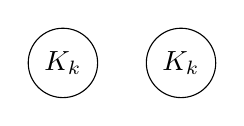
\begin{tikzpicture}
			\node[circle,draw] at (0,0){$K_{k}$};
			\node[circle,draw] at (1.5,0){$K_{k}$};
		\end{tikzpicture}
	}\]
	\caption{A disconnected graph of order $n=2k$ such that the sum of the degrees of any two nonadjacent vertices is $n-2$}
\end{figure}

Observe also that if $G$ is a disconnected graph of order $n$, then (since $G$ has at least two components) some component $G_{1}$ of $G$ has order $n_{1}$ that is at most $n/2$. Every vertex of $G_{1}$ has degree at most $n_{1}-1 \leq (n/2)-1 = (n-2)/2$ and so $\delta(G) \leq (n-2)/2$. (This observation actually provides a proof by contrapositive of Corollary 2.5.) If $G$ has three components, then the order of some component of $G$ is at most $n/3$. More generally, if $G$ has $k$ components, then the order of some component of $G$ is at most $n/k$.

The concept of degree has counterparts in both multigraphs, pseudographs and digraphs. For a vertex $v$ in a multigraph or pseudograph $G$, the \bf{degree} $\deg{}{v}$ of $v$ in $G$ is the number of edges of $G$ incident with $v$, where there is a contribution of 2 for each loop at $v$ in a pseudograph. For the pseudograph $G$ of Figure 2.4,
\begin{align*}
\deg{}{u_{1}} = 4, \deg{}{u_{2}} = 6, \deg{}{u_{3}} = 6, \deg{}{u_{4}} = 4.
\end{align*}

\begin{figure}[h]
	\caption{Illustrating degrees in a multigraph and a digraph}
\end{figure}

For a vertex $v$ in a digraph $D$, the \bf{outdegree} $\od{}{v}$ of $v$ is the number of vertices of $D$ to which $v$ is adjacent, while the \bf{indegree} $\id{}{v}$ of $v$ is the number of vertices of $D$ from which $v$ is adjacent. For the digraph $D$ of Figure 2.4,
\begin{align*}
\od{}{v_{1}} = \id{}{v_{1}} = 1, \od{}{v_{2}} = 2, \id{}{v_{2}} = 1, \od{}{v_{3}} = 0, \id{}{v_{3}} = 1.
\end{align*}

\begin{exers}\end{exers}

\begin{exer}
Give an example of the following or explain why no such example exists:
\begin{enumerate}[{(a)}]
\item a graph of order 7 whose vertices have degrees 1, 1, 1, 2, 2, 3, 3.
\item a graph of order 7 whose vertices have degrees 1, 2, 2, 2, 3, 3, 7.
\item a graph of order 4 whose vertices have degrees 1, 3, 3, 3.
\end{enumerate}
\end{exer}

\begin{exer}
Give an example of the following or explain why no such example exists:
\begin{enumerate}[{(a)}]
\item a graph that has no odd vertices.
\item a noncomplete graph, all of whose vertices have degree 3.
\item a graph $G$ of order 5 or more with the property that $\deg{}{u} \neq \deg{}{v}$ for every pair $u,v$ of adjacent vertices of $G$.
\item a noncomplete graph $H$ of order 5 or more with the property that $\deg{}{u} \neq \deg{}{v}$ for every pair $u,v$ of nonadjacent vertices of $H$.
\end{enumerate}
\end{exer}

\begin{exer}
The degree of each vertex of a certain graph of order 12 and size 31 is either 4 or 6. How many vertices of degree 4 are there?
\end{exer}

\begin{exer}
Give an example of a graph $G$ of order 6 and size 10 such that $\delta(G) = 3$ and $\Delta(G) = 4$.
\end{exer}

\begin{exer}
The degree of every vertex of a graph $G$ of order 25 and size 62 is 3, 4, 5 or 6. There are two vertices of degree 4 and 11 vertices of degree 6. How many vertices of $G$ have degree 5?
\end{exer}

\begin{exer}
Prove that if a graph of order $3n$ $(n \geq 1)$ has $n$ vertices of each of the degrees $n-1$, $n$ and $n+1$, then $n$ is even.
\end{exer}

\begin{exer}
\begin{enumerate}[{(a)}]
\item Prove that if $G$ is a bipartite graph of size $m$ with partite sets $U$ and $W$, then $m = \sum_{u \in U} \deg{}{u} = \sum_{w \in W} \deg{}{w}$.
\item Let $G$ be a bipartite graph of order 22 with partite sets $U$ and $W$, where $|U| = 12$. Suppose that every vertex in $U$ has degree 3, while every vertex of $W$ has degree 2 or 4. How many vertices of $G$ have degree 2?
\end{enumerate}
\end{exer}

\begin{exer}
Let $G$ be a graph of order $n$. If $\deg{}{u}+\deg{}{v}+\deg{}{w} \geq n-1$ for every three pairwise nonadjacent vertices $u,v$ and $w$ of $G$, must $G$ be connected?
\end{exer}

\begin{exer}
Show that if $G$ is a disconnected graph containing exactly two odd vertices, then these odd vertices must be in the same component of $G$.
\end{exer}

\begin{exer}
We have already seen that if $G$ is a graph of order $n$ such that $\deg{}{u}+\deg{}{v} \geq n-2$ for every two nonadjacent vertices $u$ and $v$ of $G$, then $G$ might be disconnected.
\begin{enumerate}[{(a)}]
\item Show that there exists a connected graph $G$ of order $n$ such that $\deg{}{u}+\deg{}{v} \geq n-2$ for every two nonadjacent vertices $u$ and $v$ and for which $\deg{}{x}+\deg{}{y}=n-2$ for some pair $x,y$ of nonadjacent vertices of $G$.
\item Let $G$ be a graph of order $n$. Prove that if $\deg{}{u}+\deg{}{v} \geq n-2$ for every pair $u,v$ of nonadjacent vertices of $G$, then $G$ has at most two components.
\item Is the bound in part (b) sharp?
\end{enumerate}
\end{exer}

\begin{exer}
Corollary 2.5 states that if $G$ is a graph of order $n$ with $\delta(G) \geq (n-1)/2$, then $G$ is connected. Is the bound $(n-1)/2$ sharp, that is, in this case, can $(n-1)/2$ be replaced by $(n-2)/2$ and obtain the same conclusion?
\end{exer}

\begin{exer}
Prove that if $G$ is a graph of order $n$ such that $\Delta(G)+\delta(G) \geq n-1$, then $G$ is connected and $diam(G) \leq 4$. Show that the bound $n-1$ is sharp.
\end{exer}

\begin{exer}
Let $G$ be a graph of order $n \geq 2$.
\begin{enumerate}[{(a)}]
\item Prove that if $\deg{}{v} \geq (n-2)/3$ for every vertex $v$ of $G$, then $G$ contains at most two components.
\item Show that the bound in (a) is sharp.
\end{enumerate}
\end{exer}

\begin{exer}
A graph $G$ has the property that every edge of $G$ joins an odd vertex with an even vertex. Show that $G$ is bipartite and has even size.
\end{exer}

\begin{exer}
A certain connected graph $G$ has the property that for every two vertices $u$ and $v$ of $G$, the length of each $u-v$ path is even or the length of each $u-v$ path is odd. Prove that $G$ is bipartite.
\end{exer}

\begin{exer}
The degree of every vertex of a graph $G$ of order $2n+1 \geq 5$ is either $n+1$ or $n+2$. Prove that $G$ contains at least $n+1$ vertices of degree $n+2$ or at least $n+2$ vertices of degree $n+1$.
\end{exer}

\begin{exer}
Let $G$ be a connected graph containing a vertex $w$ such that (1) $\deg{}{w} \centernot\equiv 0 (\mod{3})$ and (2) $\deg{}{u}+\deg{}{v} \equiv 0 (\mod{3})$ for every two adjacent vertices $u$ and $v$ of $G$. Prove that $G$ is bipartite and contains no vertex $x$ such that $\deg{}{x} \equiv 0 (\mod{3})$.
\end{exer}

\begin{exer}
Let $G$ be a graph of order 8 with $V(G) = \{v_{1},v_{2},\ldots,v_{8}\}$ such that $\deg{}{v_{i}} = i$ for $1 \leq i \leq 7$. What is $\deg{}{v_{8}}$?
\end{exer}